\chapter{Описание алгоритмов и реализации}
\section*{Повышение эффективности сборки, учитывая признак ``полезности'' при ранжировании}
\subsection*{Алгоритм}
В момент поступления url в систему, в случае её принятия хотя бы одним регулярным выражением, необходимо установить начальный ранг $c_{f}$.
\subsection*{Реализация}
Данная функциональность была реализовано при помощи двух плагинов. Первый проверяет является ли url ``полезной'', и добавляет необходимую информацию в $crawldatum$, а второй выставляет ранг согласно $crawldatum$ и настроек приложения. Такое разбиение было сделано потому что информация о том, что url является ``полезной'', представляет собой интерес и без использования данного ранжирования (например это было использовано при получении статистики).
\subsubsection*{SkaiScoringMeta}
\label{sec:scoringmeta}
SkaiScoringMeta --- плагин являющийся расширением к точке ScoringFilter, выделяющий ``полезные'' url. Для хранения дополнительной информации в $crawldatum$ используется поле $metaData$, которое представляет из себя набор пар вида $\langle key, value\rangle$
Для сохранения индикатора ``полезности'' в мета данные $crawldatum$ добавляется пара $\langle skai.scoring.fit, true\rangle$.

Для определения ``полезности'' url используется кэш с регулярными выражениями, загружаемыми из базы данных при инициализации. 

\subsubsection*{SkaiScoring}
SkaiScoring --- плагин являющийся расширением к точке ScoringFilter, выставляющий ранг. Для ссылок только что попавших в систему, зависимости от наличия мета тега, выставляет значения ранга либо $c_{f}$, либо $c_{n}$, где коэффициенты $c_{f}$ и $c_{n}$ получаются из стандартной конфигурации nutch.

\subsection*{Результат}
При использовании стандартных ScoringFilter'ов в среднем за цикл, из всех скачиваемых ссылок ``полезных'' скачивалось порядка 10\% (В качестве пространса поиска использовалось 40 крупнейших СМИ, на каждой итерации выбиралось 20000 ссылок, ``полезными'' признавались непосредственно новости). А при использовании данных плагинов уже на ранней стадии сборки порядка 80\% ссылок были ``полезными'' (Рис.~\ref{ris:img/score}). Таким образом было получено увеличение эффективности в восемь раз по сравнению с базовой реализацией nutch.

\begin{figure}[h!]
 \center{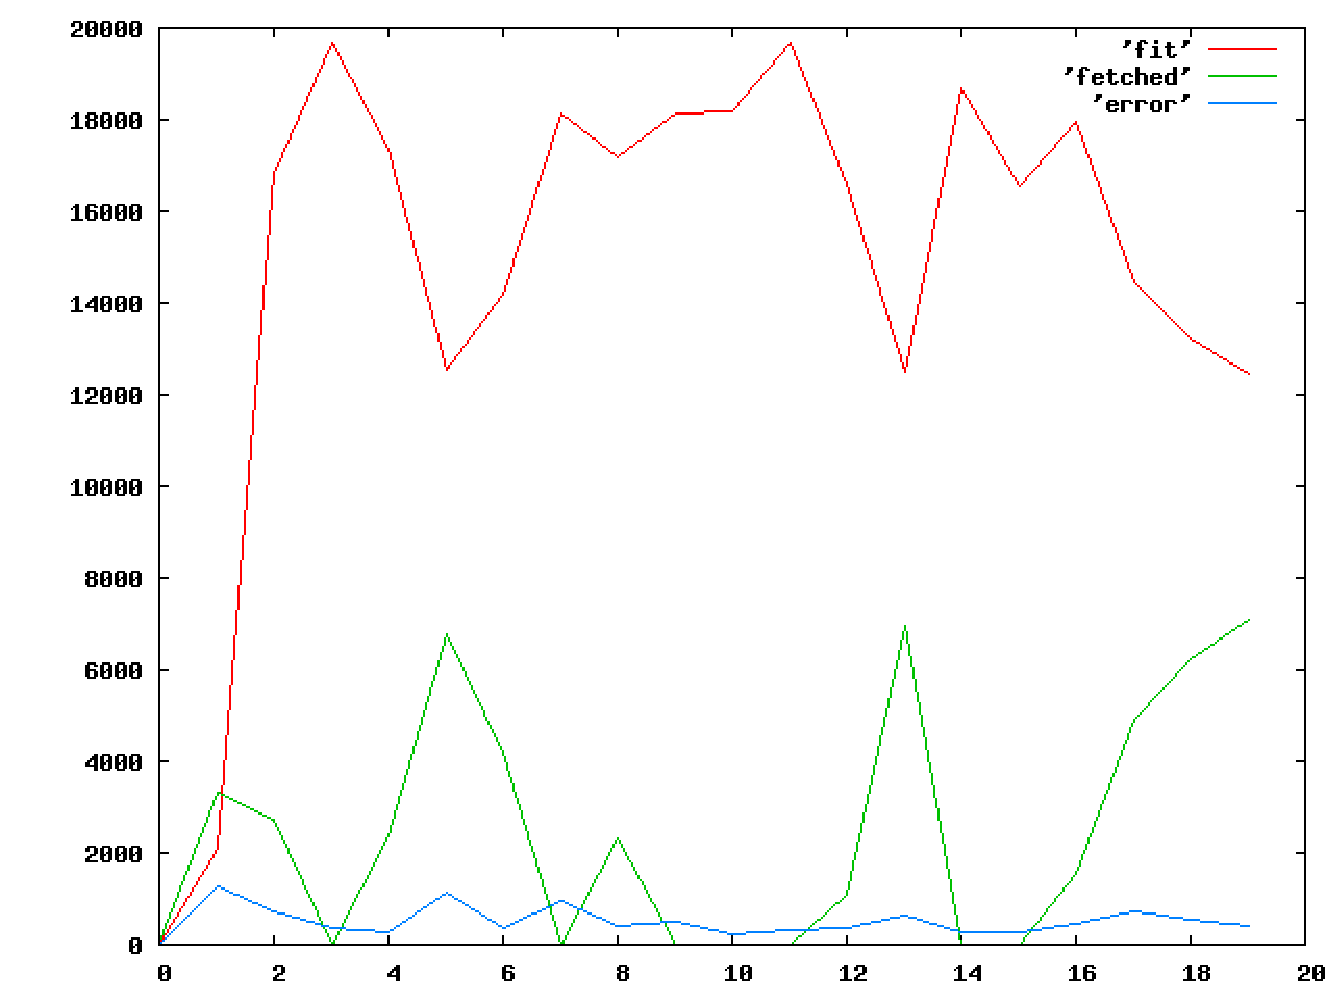
\includegraphics[width=1\linewidth]{img/scoring}}
 \caption{График зависимости числа ссылок от номера итерации. fit---число полезных ссылок, fetched---число скачанных ссылок не являющихся полезными, error---число ошибок при скачивании}
 \label{ris:score}
\end{figure}

\section*{Повышение эффективности сборки, отсечением страниц, не содержащих значимой информации}
\subsection*{Реализация фильтров}
Загрузка фильтров из базы данных является достаточно тривиальной задачей~---~во время конфигурации плагинов все фильтры загружаются не только из файлов (оставлено для совместимости с предыдущими версиями), но и из базы данных. Префиксные фильтры создаются непосредственно из описания домена, а регулярные выражения представляют из себя записи в базе данных.
\subsection*{Проблема с www}
В ходе тестирования возникла проблема --- большинство ресурсов по url вида \ref{eq:domain} и \ref{eq:wwwdomain} содержат один и тот же документ, как правило отличающийся тем что в первом документе все исходящие url содержат www, а во втором нет.
\begin{equation} \label{eq:domain}
 http://domainname/documentname
\end{equation}

\begin{equation} \label{eq:wwwdomain}
 http://www.domainname/documentname
\end{equation}


Что бы избежать дублирования документов, разумно фильтровать либо ссылки с www, либо без www.

Однако бывают ресурсы в которых из документа с url вида \ref{eq:domain} присутствуют как ссылки с www так и без, таким образом часть нужных ссылок выбрасывается фильтрами. Для решения подобной проблемы пришлось модифицировать нормализатор url.
\subsubsection*{Нормализатор url}
Нормализатор url (url normalizer) --- точка расширения nutch (URLNormalizer), которая отвечает за преобразование url на различных стадиях работы. В nutch реализовано несколько нормализаторов, которые подобно ScoreFilter'ам обьеденены в цепь. Так же URLNormalizer предоставляет возможность использовать разные правила преобразования на разных этапах сборки.

Для решения возникшей проблемы за основу был взят стандартный RegexUrlNormalizer, который осуществляет преобразование url по средствам регулярных выражений. Было добавлено создание правил заменяющих url с www на url без www, если домен был помечен как ``без www'' и наоборот в противном случае.

\section*{Получение статистики}
Основная идея заключается в том, что бы получить записи вида $\langle domain,prefix,metrics \rangle$ где:
\begin{itemize}
 \item domain --- домен к которому относится запись.
 \item prefix --- префикс url к которому относится запись.
 \item metrics --- набор пар вида $\langle state, count\rangle$, где $count$ --- это число документов с данным префиксом на данном домене, в состоянии $state$ (например: новая ссылка, скачанная ссылка, ``полезная ссылка'').
\end{itemize}
По подобным записям в дальнейшем достаточно легко делать выводы о разделах ресурсов.
\subsection*{Алгоритм}
Поскольку данная задача работает с crawldb, размер которой может быть очень большим, алгоритм необходимо представить в виде  \nameref{sec:mapred} задачи.

\subsubsection*{Map}
На этапе map по $url$ и $crawldatum$ получается множество пар $\langle prefix,info\rangle+$, где $prefix$ это префикс url вместе с доменом, а $info$ это пара вида $\langle state,1\rangle$
$$\langle url, crawldatum \rangle \rightarrow \langle prefix,info\rangle+ $$

Сначала из $url$ неким способом получается множество префиксов $S_{p}$, например:
$$ http://lenta.ru/2010/05/09/ \rightarrow $$
$$ http://lenta.ru/2010/05/09, $$
$$ http://lenta.ru/2010/05/, $$
$$ http://lenta.ru/2010/, $$
$$ http://lenta.ru/; $$


Далее в зависимости от свойств $url$ описанных в $crawldatum$ создается множество метрик $S_{m}$, например если ссылка была ``полезной'' но не была еще скачана, то $$ S_{m}=\{\langle fit,1\rangle, \langle unfetched,1\rangle\}$$

Затем все пары из $S_{p} \times S_{m}$ попадают в выходной поток. Для эффективной работы необходимо, что бы $url$ разбивалось на наименьшее число префиксов, но так, что бы основные разделы домена могли быть сопоставлены какому-нибудь префиксу. В идеале множество метрик может содержать только одно значение, если $url$ не может находится сразу в нескольких состояниях.
\subsubsection*{Reduce}
На этапе reduce метрики префиксов суммируются и отбрасываются незначительные префиксы
$$\langle prefix,\langle state,1\rangle+\rangle \rightarrow \langle prefix,metricvector\rangle$$

$Metricvector$ представляет из себя вектор из пар $\langle state, nurl \rangle$, где $nurl$ --- число $url$ c состоянием $state$.
Незначительными признаются метрики где сумма $nurl$ достаточно мала. Такие префиксы отбрасываются, а остальные сохраняются в базу данных.

\subsection*{Реализация}
В ходе реализации был изменен класс CrawlDbReader, отвечающий за получение статистики. Написаны классы для map и reduce.

\subsubsection*{CrawlDbExtendedStatMapper}
CrawlDbExtendedStatMapper --- класс имплементирующий стандартный интерфейс \nameref{sec:hadoop} --- Mapper, который служит для создания собственных этапов map.
Для разбиения url на префиксы был использован UrlSplitter, который разбивал url на не более чем $n_{s}$ префиксов по символу ``/'', так же как и в примере с lenta.ru. Таким образом $|S_{p}|\leqslant n_{s}$ Пожалуй это самая простая реализация которая требует доработки в будущем.
В качестве метрик использовались следующие показатели:
\begin{itemize}
 \item unfetched ---документ по ссылке не был скачан.
 \item fetched --- документ по ссылке была скачана.
 \item fit --- ссылка была признана ``полезной''
\end{itemize}
Первые два показателя брались непосредственно из статуса $crawldatum$, а последняя из мета данных, которые были проставлены с помощью \nameref{sec:scoringmeta}. Таким образом $|S_{m}|\leqslant2$. В результате число записей попадающих в выходной поток $n\leqslant 2\cdot n_{s}\cdot n_{url}$, где $n_{url}$ --- число записей в crawldb.

\subsubsection*{CrawlDbExtendedStatReducer}
CrawlDbExtendedStatReducer --- класс имплементирующий стандартный интерфейс \nameref{sec:hadoop} --- Reducer, который служит для создания собственных этапов reduce.

На этапе reduce суммируются все показатели для префикса и если $n_{unfetched}+n_{fetched} < n_{s}$ префикс отбрасывается. Для совместимости со стандартным CrawlDbReader'ом и уменьшения нагрузки на базу данных, префиксы не сразу добавляются в базу данных, а выводятся в файл. 
\subsubsection*{Добавление в базу данных}
После отработки MapReduce работы, её результат считывается из файла, после чего все записи добавляются в базу данных одним запросом. Так же в базу передается время в которое статистика была создана.

Получать статистику можно достаточно редко --- например один раз в 5-20 циклов, таким образом, время на сбор статистики не оказывает существенного влияния на эффективность.
\subsection*{Результаты}
Для crawldb c 10 000 000 url время получения статистики составляет порядка 15\% от общего времени работы цикла с 20 000 ссылок. Таким образом, при создании статистики каждый двадцатый цикл, потеря времени составляет порядка 0.75\%, которой  можно пренебречь.

\section*{Генерация фильтров}
При создании алгоритма были сделаны следующие предположения:
\begin{itemize}
 \item все ``полезные'' можно ограничить некотором числом разделов, не зависящем от числа документов. (под разделом понимается некий префикс url)
 \item архив документов находится в определенном разделе (под архивом понимаются документы с ссылками на ``полезные'' документы)
 \item архив достижим из корневого документа
 \item документов архива меньше чем ``полезных''
\end{itemize}

\subsection*{Алгоритм}
Сам алгоритм, пользуясь некоторой эвристикой, признает некоторые префиксы ненужными, из которых потом создаются фильтры.
Простейший алгоритм выбирающий префиксы согласно сделанным предположениям выглядит так:
\begin{enumerate}
 \item Выбирается вся статистика для конкретного домена.
 \item Домены для которых $u_{d}<n_{d}$ далее не рассматриваются.
 \begin{itemize}
  \item $u_{d}$ --- число ``полезных'' ссылок во всем домене
  \item $n_{d}$ --- пороговое значение, введенное для того, что бы не начать создавать фильтры до того, как будут получены ссылки на архив.
 \end{itemize}

 \item По префиксам для которых $u_{p}=0$ и $s_{p}>u_{d}$ создаются исключающие правила.
 \begin{itemize}
  \item $u_{p}$ --- число ``полезных'' ссылок с данным префиксом
  \item $s_{p}$ --- общее число известных ссылок с данным префиксом
 \end{itemize}
 Сам по себе префикс уже представляет из себя префиксный фильтр.
\end{enumerate}


\subsection*{Реализация}
Данная функциональность была реализована в виде отдельного приложения запускающегося сразу после создания статистики. Поскольку пользовательские фильтры были организованы на базе RegexURLFilter, для простоты управления автоматически созданные фильтры были тоже реализованы регулярными выражениями. 

Была предусмотрена возможность отключения конкретного фильтра таким образом, что бы он не создавался заново. Для этого фильтр не удалялся из базы данных, а просто становился не активен.

\subsection*{Результат}
Качество результатов работы данного алгоритма достаточно сложно оценить, однако на тестовых данных автоматические фильтры достаточно успешно находили бесполезные разделы. Предполагается что существенное увеличение производительности будет получено на позднем этапе сборки - когда большая часть ``полезных'' документов уже будет скачена.
